\documentclass[border=2pt]{standalone}
\usepackage{tikz}
\usetikzlibrary{positioning, arrows.meta, calc, fit}
\begin{document}
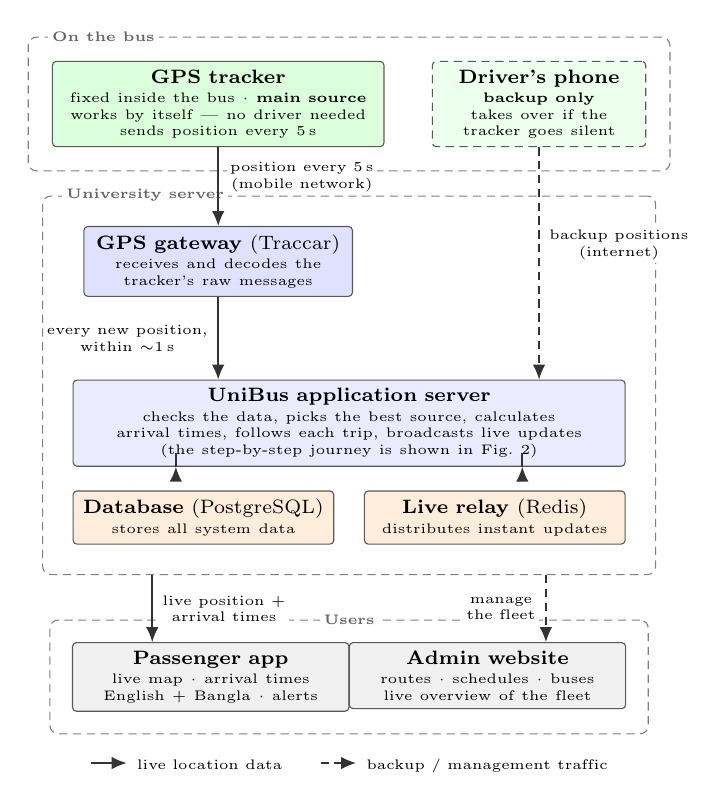
\begin{tikzpicture}[
  font=\scriptsize,
  arr/.style={-{Latex[length=1.9mm,width=1.6mm]}, semithick, draw=black!80},
  barr/.style={-{Latex[length=1.9mm,width=1.6mm]}, semithick, draw=black!80, densely dashed},
  blk/.style={draw=black!65, rounded corners=1.4pt, align=center, inner sep=3pt, fill=white},
  lab/.style={font=\tiny, align=center, inner sep=1.2pt, fill=white},
  zone/.style={draw=black!50, densely dashed, rounded corners=3pt, inner sep=3.8mm},
  zlab/.style={font=\tiny\bfseries\scshape, text=black!60, fill=white, inner sep=1.5pt}
]
% ================= ON THE BUS =================
\node[blk, fill=green!14, text width=40mm] (gt)
  {\textbf{GPS tracker}\\[-1pt]
   {\tiny fixed inside the bus $\cdot$ \textbf{main source}}\\[-2pt]
   {\tiny works by itself --- no driver needed}\\[-2pt]
   {\tiny sends position every 5\,s}};
\node[blk, fill=green!7, densely dashed, text width=25mm,
      anchor=north west] (ph) at ($(gt.north east)+(6mm,0)$)
  {\textbf{Driver's phone}\\[-1pt]
   {\tiny \textbf{backup only}}\\[-2pt]
   {\tiny takes over if the}\\[-2pt]
   {\tiny tracker goes silent}};
\node[zone, fit=(gt)(ph), inner sep=3mm] (vzone) {};
\node[zlab, anchor=west] at ($(vzone.north west)+(2.5mm,0)$) {On the bus};

% ================= SERVER =================
\node[blk, fill=blue!12, text width=32mm, below=10mm of gt] (trac)
  {\textbf{GPS gateway} (Traccar)\\[-1pt]
   {\tiny receives and decodes the}\\[-2pt]
   {\tiny tracker's raw messages}};
\node[blk, fill=blue!8, text width=68mm, anchor=north]
  (app) at ($(vzone.center |- trac.south)+(0,-10.5mm)$)
  {\textbf{UniBus application server}\\[-1pt]
   {\tiny checks the data, picks the best source, calculates}\\[-2pt]
   {\tiny arrival times, follows each trip, broadcasts live updates}\\[-2pt]
   {\tiny (the step-by-step journey is shown in Fig.~2)}};
\node[blk, fill=orange!14, text width=31mm, below=3mm of app.south west, anchor=north west] (pg)
  {\textbf{Database} (PostgreSQL)\\[-1pt]{\tiny stores all system data}};
\node[blk, fill=orange!14, text width=31mm, below=3mm of app.south east, anchor=north east] (rd)
  {\textbf{Live relay} (Redis)\\[-1pt]{\tiny distributes instant updates}};
\draw[arr] ($(app.south)+(-22mm,0)$) -- ($(app.south)+(-22mm,0)$ |- pg.north);
\draw[arr] ($(app.south)+(22mm,0)$) -- ($(app.south)+(22mm,0)$ |- rd.north);
\node[zone, fit=(trac)(app)(pg)(rd)] (svzone) {};
\node[zlab, anchor=west] at ($(svzone.north west)+(2.5mm,0)$) {University server};

% ================= USERS =================
\node[blk, fill=black!6, text width=33mm, anchor=north west] (pass)
  at ($(svzone.south west)+(3.8mm,-8.5mm)$)
  {\textbf{Passenger app}\\[-1pt]
   {\tiny live map $\cdot$ arrival times}\\[-2pt]
   {\tiny English $+$ Bangla $\cdot$ alerts}};
\node[blk, fill=black!6, text width=33mm, anchor=north east] (adm)
  at ($(svzone.south east)+(-3.8mm,-8.5mm)$)
  {\textbf{Admin website}\\[-1pt]
   {\tiny routes $\cdot$ schedules $\cdot$ buses}\\[-2pt]
   {\tiny live overview of the fleet}};
\node[zone, fit=(pass)(adm), inner sep=2.8mm] (uzone) {};
\node[zlab] at (uzone.north) {Users};

% ================= ARROWS =================
\draw[arr] (gt.south) -- (trac.north)
  node[lab, pos=0.38, anchor=west, xshift=1mm] {position every 5\,s\\(mobile network)};
\draw[barr] (ph.south) -- (ph.south |- app.north)
  node[lab, pos=0.42, anchor=west, xshift=0.8mm] {backup positions\\(internet)};
\coordinate (tD) at (trac.south);
\draw[arr] (tD) -- (tD |- app.north)
  node[lab, midway, anchor=east, xshift=-0.8mm] {every new position,\\within $\sim$1\,s};
\coordinate (pA) at ($(svzone.south west)+(14mm,0)$);
\coordinate (aA) at ($(svzone.south east)+(-14mm,0)$);
\draw[arr] (pA |- svzone.south) -- (pA |- pass.north)
  node[lab, midway, anchor=west, xshift=0.8mm] {live position $+$\\arrival times};
\draw[barr] (aA |- svzone.south) -- (aA |- adm.north)
  node[lab, midway, anchor=east, xshift=-0.8mm] {manage\\the fleet};

% ================= LEGEND =================
\node[anchor=north, font=\tiny] at ($(uzone.south)+(0,-1.6mm)$)
  {\tikz{\draw[arr] (0,0) -- (4.5mm,0);}\, live location data\qquad
   \tikz{\draw[barr] (0,0) -- (4.5mm,0);}\, backup / management traffic};
\end{tikzpicture}
\end{document}
